\subsubsection{Последовательная диаграмма работы модуля Chats}
Модуль «Chats» обеспечивает обмен сообщениями в реальном времени между пользователями системы (преподавателями и студентами) посредством WebSocket-соединения. Ниже на рисунке~\ref{fig:chats-flow} приведена последовательная диаграмма, демонстрирующая ключевые этапы работы чата: открытие приложения, выбор беседы, отправка и приём сообщений, а также обработку истечения JWT и повторное подключение.

\begin{figure}[H]
    \centering
    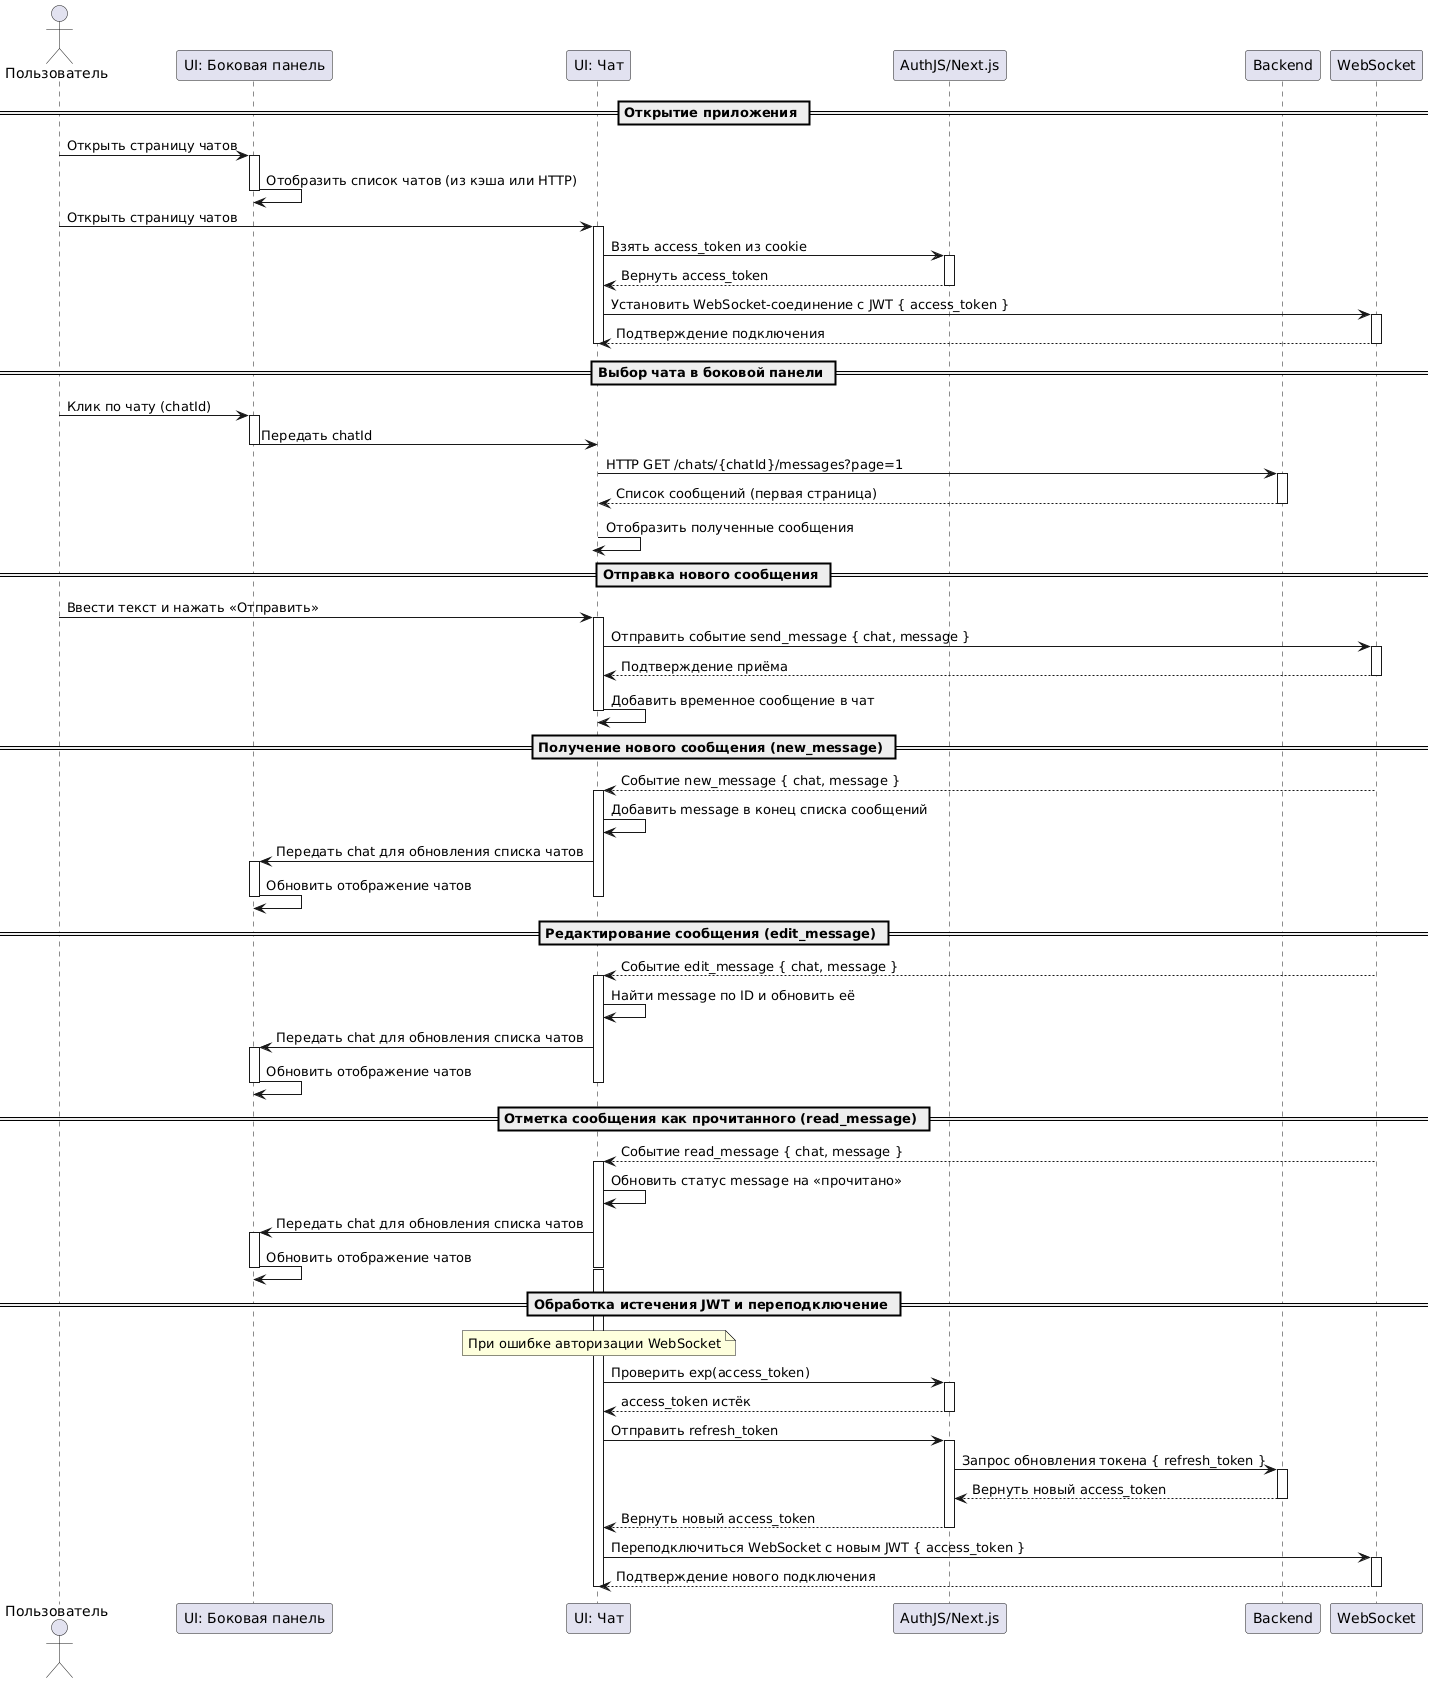
\includegraphics[width=0.9\textwidth]{static/diagrams/Chats.png}
    \caption{Схема взаимодействия клиента (UI: Боковая панель и UI: Чат), AuthJS (Next.js), бэкенда и WebSocket при работе модуля «Chats».}
    \label{fig:chats-flow}
\end{figure}

На рисунке~\ref{fig:chats-flow} выделены следующие этапы:

\begin{enumerate}
    \item \textbf{Открытие приложения:}
    \begin{itemize}
        \item Пользователь переходит в раздел «Чаты». UI боковой панели запрашивает и отображает список доступных бесед (из кэша или по HTTP).
        \item При загрузке страницы «Чат» UI извлекает \texttt{access\_token} из защищённой cookie (AuthJS).
        \item После получения токена устанавливается WebSocket-соединение с сервером, передавая JWT в заголовке. Бэкенд подтверждает подключение.
    \end{itemize}

    \item \textbf{Выбор чата в боковой панели:}
    \begin{itemize}
        \item Пользователь кликает на одну из бесед (параметр \texttt{chatId}). Боковая панель передаёт этот \texttt{chatId} компоненту «Чат».
        \item UI «Чат» выполняет HTTP GET-запрос к эндпоинту \texttt{/chats/\{chatId\}/messages?page=1} для получения первой страницы сообщений.
        \item Бэкенд возвращает список сообщений, которые UI отображает в области истории сообщений.
    \end{itemize}

    \item \textbf{Отправка нового сообщения:}
    \begin{itemize}
        \item Пользователь пишет текст сообщения и нажимает «Отправить» в UI «Чат».
        \item UI «Чат» эмиттит событие \texttt{send\_message} по WebSocket, передавая объект \{\texttt{chat: chatId, message: {…}}\}.
        \item Бэкенд принимает событие, сохраняет сообщение и возвращает подтверждение приёма.
        \item UI «Чат» временно отображает отправленное сообщение (optimistic UI) со статусом “отправляется” до получения фактического сообщения от сервера.
    \end{itemize}

    \item \textbf{Получение нового сообщения (\texttt{new\_message}):}
    \begin{itemize}
        \item Когда любой участник (в том числе другой пользователь) отправляет сообщение, сервер по WebSocket рассылает событие \texttt{new\_message} всем подписанным участникам данного чата.
        \item UI «Чат» получает событие \texttt{new\_message \{ chat, message \}} и добавляет новое сообщение в конец списка истории.
        \item Боковая панель получает обновлённый \texttt{chatId} для обновления списка бесед (например, переставить текущую беседу наверх) и отображает актуальный список чатов с учётом новых сообщений.
    \end{itemize}

    \item \textbf{Редактирование сообщения (\texttt{edit\_message}):}
    \begin{itemize}
        \item Если пользователь (автор сообщения) редактирует ранее отправленное сообщение, UI «Чат» отправляет серверу по WebSocket событие \texttt{edit\_message \{ chat, message \}}.
        \item Сервер обновляет текст сообщения и рассылает событие \texttt{edit\_message} всем участникам беседы.
        \item UI «Чат» находит сообщение по его \texttt{id} или \texttt{local\_id} и обновляет текст.
        \item После этого боковая панель получает сигнал «передать chatId» для обновления порядка бесед и отображает обновлённый список чатов.
    \end{itemize}

    \item \textbf{Отметка сообщения как прочитанного (\texttt{read\_message}):}
    \begin{itemize}
        \item Когда пользователь прокручивает историю и дожидается видимости новых сообщений, UI «Чат» отправляет событие \texttt{read\_message \{ chat, message \}} по WebSocket.
        \item Сервер обновляет статус сообщения на «прочитано» и уведомляет других участников через событие \texttt{read\_message}.
        \item UI «Чат» и боковая панель получают это событие, обновляют статус соответствующего сообщения и обновляют отображение списка чатов (например, убрать бейдж «новых сообщений»).
    \end{itemize}

    \item \textbf{Обработка истечения JWT и переподключение:}
    \begin{itemize}
        \item Если при работе WebSocket возникает ошибка авторизации (например, \texttt{access\_token} истёк), UI «Чат» получает событие \texttt{connect\_error} от библиотеки Socket.IO.
        \item Компонент проверяет поле \texttt{exp(access\_token)} локально. При истечении:
        \begin{enumerate}
            \item UI «Чат» отправляет \texttt{refresh\_token} на AuthJS/Next.js, получая новый \texttt{access\_token}.
            \item После получения нового токена выполняется повторное подключение WebSocket, передавая обновлённый JWT.
            \item Сервер WebSocket подтверждает новый сеанс подключения.
        \end{enumerate}
        \item Боковая панель и UI «Чат» возобновляют подписку на события и продолжают обмен сообщениями без потери данных.
    \end{itemize}
\end{enumerate}

Таким образом, последовательная диаграмма на рисунке~\ref{fig:chats-flow} отражает полный цикл работы модуля «Chats»: от открытия приложения и установления защищённого соединения до приёма, отправки, редактирования и пометки сообщений, а также автоматического обновления JWT и переподключения WebSocket. Все события обрабатываются как в компоненте UI «Чат», так и в боковой панели, чтобы гарантировать актуальность списка бесед и статусов сообщений.
